\section{Experiment}
\label{sec:experiment}
%In this paper, our task is to tackle commonsense reasoning problem in stories. 
%Given SCT as evaluation set, we can use any source data to learn human commonsense knowledge and reasoning ability. 
%We suppose the validation data has information leak for test set. The most classification methods which training or fine tuning with SCT validation set may learn the bias leak features, rather than commonsense reasoning ability
We first introduce some competing methods to be evaluated as well as
the datasets that they used for training and testing.
Then we present a preliminary analysis on the ROCStory dataset to invalidate
previous approaches that train or fine tune their models on the validation
set. Finally we present a comprehensive
evaluation of the competing methods.

%In this paper, our task is to tackle commonsense reasoning problem in stories. 
%Given SCT as evaluation set, we can use any source data to learn human commonsense knowledge and reasoning ability. 
%We suppose the validation data has information leak for test set. The most classification methods which training or fine tuning with SCT validation set may learn the bias leak features, rather than commonsense reasoning ability(\secref{sec:dataset}). We suggest to use a larger corpus with negative ending generated automatically. We also show our model parameter details in \secref{sec:details}, the comparison result with analysis in \secref{sec:result} and ablation study is in \secref{sec:ablation} .
\subsection{Baselines and our method}
\label{sec:baselines}
We compare our model with previous work on SCT task including the 
state-of-art methods: 

\begin{description}
\item[SIMP]~\cite{srinivasan2018simple} uses skip thought embeddings and 
encodes the entire context using several Dense layers to train 
a classifier to determine the right ending.

\item[SKBC]~\cite{roemmele2017rnn} is similar to SIMP using skip thought 
embedding trained with different source and a GRU neural network to 
train a binary classifier.

\item[DSSM]~\cite{mostafazadeh2016corpus} which performs the best 
among original baselines by calculating  the similarity between the 
context sentence vector and ending vector.

\item[CGAN]~\cite{wang2017conditional} use an generative adversarial 
networks (GAN) which apply GRU to generate negative endings for 
training data augment.

\item[SeqMANN]~\cite{li2018multi} takes multiple shallow features in 
to account, including POS tag, word character, char character, 
sentiment negation and SemLM~\cite{peng2016two} features.

\item[FTLM]~\cite{radford2018improving} make a big improvement by using 
multi-layer transformer to train a language model for text representation 
with linear fine tuning.

\item[ISCK]~\cite{chen2018incorporating} incorporates  sentiment and 
commonsense feature between the context and ending to 
\citeauthor{radford2018improving}'s text representation which can get a little improvement.

\item[GMSA]~\cite{guan2018story} generates the story ending through 
multi-source attention and take in ConceptNet neighboring information.
\end{description}

%In \textbf{our model}, the sentence representation contains text sentence 
%representation and commonsense structured representation. 
Because the Roemmele~\cite{roemmele2017rnn} has shown that training 
sentence representation using ROCStories is almost as effective as
using BookCorpus, for {\bf our model}, we choose to train the
concept sequence representation  
using a 2400-dimensional language model\cite{kiros2015skip} 
from 98,161 unannotated ROCStories instead of using
the larger BookCorpus. 

The structured knowledge representation takes form of a 
300-dimensional vector. 
%For the tuning hyper parameter on story ending classifier. 
%We combine the sentence representations of the context and 
%final sentence into one sequence. 
Each sentence representation is fed through a dropout layer 
(drop-rate of 0.4) and further fed into a single 1000-node 
GRU hidden layer. 
%The final hidden state value of two samples with same 
%context are given to a top feed-forward layer composed of one node  
%with softmax activation. 
A binary cross-entropy objective function is 
applied to train the network. All experiments use a batch size of 
200 to optimize the model over 30 training epochs. 


\subsection{Dataset}
\label{sec:dataset}

\begin{table}[th]
\small
\begin{tabular}{lllll} \hline
\bf{Methods} & LM Train & Pred. Train & Validation & Test \\ \hline \hline
SIMP & BC & ROCS*(T)& ROCS*(V)& SCT \\ \hline
SKBC & ROCS & ROCS*(T)& ROCS*(V)& SCT\\ \hline
DSSM & ROCS & -  & - &  SCT\\ \hline
CGAN & ROCS & - & - &  SCT\\ \hline
SeqMANN & ROCS & ROCS*(T)& ROCS*(V)& SCT\\ \hline
FTLM & BC &  ROCS*(T)& ROCS*(V)& SCT\\ \hline
ISCK & BC + ROCS & ROCS*(T) & ROCS*(V) & SCT \\ \hline
GMSA & ROCS & - & - & SCT \\ \hline
Ours & ROCS &ROCS*(T) &ROCS*(V) & SCT \\ \hline
\end{tabular}
\caption{Datasets used by different methods for training
language model and the ending prediction, for validation and
for test
(BC = BookCorpus,
ROCS = ROCStories, ROCS* = ROCStories annotated with positive and 
negative endings by AMT,
SCT=Story Cloze Test)}
\label{tab:datasets}
\end{table}

All datasets used in the experiments are documented in
\tabref{tab:datasets}. BookCorpus contains text from
11,038 books, primarily novels.  
ROCStories corpus consist of 98,161 unannotated five-sentence 
stories. BookCorpus and ROCStories have been used to pre-train
language models for this task in the past.

To train the story ending prediction models, many previous works
used the SCT validation split which contains 1871 annotated items,
and achieved very good results.
We argue that the validation set cannot be used as training resource because
it suffers from human-authorship bias~\cite{sharma2018tackling}.  
The following preliminary experiment show why. 

ROCStories and their negative endings in SCT are solicited
on Amazon Mechanical Turk (AMT). We found that the endings
contain significant information leak. For example, \tabref{tab:hate}
shows a feature (the word ``hate'') that is overwhelmingly found 
in the negative endings.
This means that by extracting such features from two endings, an algorithm
maybe able to predict the correct ending with high accuracy. 

\begin{table}[th!]
\small
\centering
\begin{tabular}{lccc}
\hline
  & Pos ending& Neg ending &Total\\
\hline
Validation set & 3  & 70 &73\\
Test set          & 4  & 69 &73\\
\hline
\end{tabular}
\caption{Frequency of word ``hate'' appearing in the positive and 
negative endings of SCT Validation set and Test set}
\label{tab:hate}
\end{table}

We re-evaluated several top-performing algorithms and our method
by adapting them to training {\em only on the endings} in the validation set. 
The result on the test set of SCT is shown in \tabref{tab:end}. 
As a baseline, we include the human performance, which is the average
accuracy of 5 human annotators. Note that the human annotators are not
trained on the validation set but use their commonsense only. The fact
that humans score substantially worse than some of the ``top'' algorithms
indicates that these algorithms are not using ``commonsense'' but rather
the patterns leaked in the training data. 

\begin{table}[th!]
\small
\centering
\begin{tabular}{lcc}
\hline
\textbf{Model}& SCT (\%) &ROCS*(T) (\%)\\
\hline
%~\citeauthor{end:predict}(~\citeyear{end:predict})&72.5\\
SIMP& 72.60 &59.86\\
SKBC&72.76&58.18\\
FTLM& 77.77 &57.93\\
Our model& 68.74&58.98\\
\hline
Human& 62.40&62.40\\
\hline
\end{tabular}
\caption{Test accuracies of various models train on the endings only
from SCT validation and ROCS*(T)}
\label{tab:end}
\end{table}

Therefore, in this paper, we choose to create a new training dataset
by automatically augmenting ROCStories corpus with negative endings.
We do this because it is unnatural for humans to come up with negative
endings for a story, while most people have no problem predicting a positive
one.
We propose to generate negative endings automatically \cite{roemmele2017rnn}. 
We generate negative examples for the 98161 stories in ROC training set 
by Random and Backward method with 4:2 proportion. The resulting dataset
is called ROCS*.
Finally, we split ROCS* 4:1 into training (ROCS*(T)) and 
validation set (ROCS*(V)) for the end-to-end training and validation. 
%The second reason for why we don't use validation for training is the quantity of the SCT validation set. It only contains 1871 stories. Most of the previous research split 1497 stories for training and 376 stories for validating. Intuitively, learning the ability of commonsense reasoning in story from about 1500 stories is impossible. \KZ{Can we have a bit of result here to support thisclaim? There are two reasons u present here but the second one is too light-weight.} 

%\KZ{The following 3 paragraphs are too verbose. Cut to just one short para!} 
%The motivation of this task is to learn large quantity of commonsense knowledge and reasoning ability. Given SCT evaluation dataset, most of previous research are trained with negative examples. However, writing large amount of negative examples manually is too expensive. At the same time, human writing  always take in human bias, just as the example in ~\tabref{tab:end}.
%
% Because story ending should initially have two features: probability equivalence and coherence. In ROC validation set, some endings are illogical in commonsense, for example, the ending ``the glasses fixed his headaches immediately'' is much more likely than``the optometrist gave him comfortable sneakers''. Of course, the second ending is wrong, but the inequity  have nothing to do with story prediction task. We choose the endings from other story which are equal in probability. In addition, the backward approach improves the degree of semantic coherence with the context sentences. 
%
%We shuffle and split the 98161 story set with negative endings into 5 folds, one for  Valid-RB (new validation set) and the rest for Train-RB (new training set). The test set is the same with SCT. The accuracy for models train on Train-RB endings is shown in  ~\tabref{tab:end}. By comparison with \tabref{tab:end}, the scores imply the models can not get a good model with only endings. Train-RB strongly reduces the ending bias.
%
%
%%\KZ{You need to add a paragraph to talk about how you evaluated human
%performance. Who participated in these test, how were they evaluated.
%Maybe the same humans did the test for the endings only. So we need to
%think about where to put this paragraph. Here or earlier when you talk
%about ending only.}
 
\subsection{Results}
\label{sec:result}

\begin{table}[th]
 \small
\centering
\begin{tabular}{lc}
\hline
$\textbf{Unsupervised}$ & Acc (\%)\\
\hline
DSSM& 58.50\\
GMSA& 61.20\\
\hline
$\textbf{Semi-supervised}$ & Acc (\%)\\
\hline
CGAN& 60.90 \\
SIMP&61.09\\
SKBC&64.70\\
SeqMANN& 59.74\\
FTLM& 63.46 \\
ISCK& 62.21 \\
Our model& {\bf 69.70}\\
\hline
Human& 100\\
\hline
\end{tabular}
\caption{End-to-end accuracy on SCT test set}
\label{tab:all-models}
\end{table}

\tabref{tab:all-models} shows results from the baselines and our model on 
SCT test set. 
%We use the same training data for
%all supervised or semi-supervised approaches in this section. 
%\footnote{Some of the algorthms compared here may have reported better
%accuracies than those reported here, but that's because they were trained
%on the validation set.}
Human performance is 100\% and can be used as an 
upperbound~\cite{mostafazadeh2016corpus}. The models are divided into two
categories, namely semi-supervised and unsupervised, which either use
the generated negative endings or not at all. All results are averaged from
5 independent runs.

%DSSM achieves an accuracy of 58.5\%, it simply uses a deep structured semantic model to learn representations for both context and endings and chose ending by calculating the similarity between the context and ending representation. GMSA model is a generative model, which takes in structured ConceptNet knowledge. Though it is not used for choosing endings, we compute the similarity between the generated ending and two alternatives and get 61.2\% for comparison. The semi-supervised models all rely on negative endings. CGAN achieves 60.9\% accuracy by generating negative endings with generator in GAN. The goal of their generator network is to generate a fake sentence and deceive the discriminator to take it as real target. SeqMANN achieves 59.74\% accuracy incorporating with many language features,. FTLM make great achievement training on SCT validation set and get 63.46\% accuracy training on Train-RD. This model use transformer train a language model and fine tune to train a classifier. ISCK which is the best when using SCT validation set for training further improves the performance to 62.21\%. It combines the sentence representation of FTLM, sentiment feature and commonsense similarity feature between the context and endings. SKBC the state-of-art in former models we reproduce achieves 64.7\% accuracy with skip-thought sentence representation and RNN classifier. We suppose FTLM and ISCK learn the representation of sentence itself. Skip-thought model encode the sentence representation with former and later sentence information. This kind of information is more efficient in commonsense reasoning. SIMP is even more simple for only using dense layer to classify the story lines on 61.09\% accuracy. 
 
Our model outperforms all the baselines. In fact we 
logged 5\% improvement over
RNN-BC which was the previous state-of-the-art. 
%Similar to SKBC model, we represent the story sentence with 
%low-dimension vectors and train a classifier with GRU model. 
Our improvement comes from our simplification and commonsense feature 
incorporation. There exists 43,095 unique words in all ROCStories and 
19455 unique words in simplified key tokens extracted from ConceptNet. 
This greatly reduces the noise and variance in sequential sentence 
representation training. In addition, the structured commonsense feature 
also takes extra commonsense knowledge.

Also, for the record, our model correctly predicts the question in
\figref{fig:story} while other strong competitors such as SIMP, FTLM and ISCK
failed.

%\KZ{Add one or two example stories in which we did correct but other algorithms
%failed. Give a brief analysis to show why our method do better 
%than this example. Actually here it would be ideal if our driving example
%can be used. That is, indeed our method predicts correctly while the major
%competitors failed.}
 
\subsection{Ablation Study}
\label{sec:ablation}
%Previous work on predicting ending of a story mainly divided into two directions. The first direction aims to generate ending for given context with generative language model~\cite
\begin{table}[th!]
\small
\centering
\begin{tabular}{lc}
\hline
\textbf{Types of information} & Acc (\%)\\
\hline \hline
SKBC (whole sentence embedding)& 64.70 \\
\hline
Ours (only simplified sentence embedding)& 68.13 \\
Ours (only concept embedding)&  63.70\\
\hline
Ours (SSE+CE)& {\bf 69.70}\\
\hline
\end{tabular}
\caption{The effect of using different types of embedding}
\label{tab:ablation}
\end{table}

\begin{figure}[th!]
\centering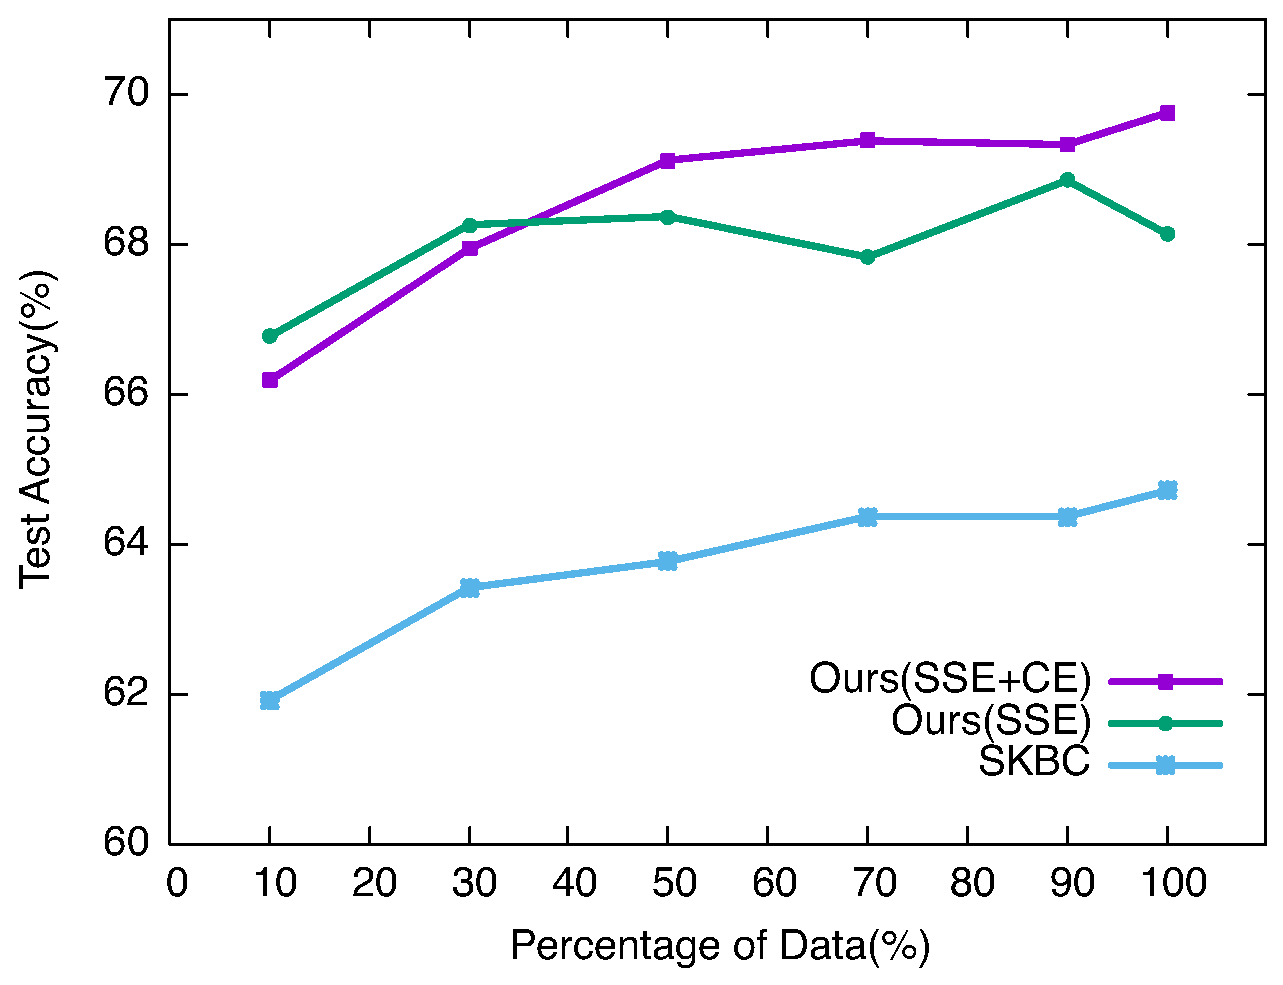
\includegraphics[width=0.8\columnwidth]{pictures/trend}
\caption{Accuracies over train data size}\label{fig:trend}
\end{figure}

We conduct an ablation study on the proposed model to evaluate 
the effectiveness of each feature. Results using only one type of 
embedding for sentence representation are shown in \tabref{tab:ablation}. 
The representation with simplified sentence achieves 3.43\% improvement 
over the sentence embedding of the original sentence. It also shows that
sentence simplification is a more effective feature than concept embedding. 

In \figref{fig:trend}, we compare the models' capability given increasing
amount of training data. The first observation is that our two models (SSE+CE
and SSE) both perform strongly even with very little training data. In fact,
at 10\% of the data, they already achieve better accuracies than SKBC using
the whole data. The second observation is that compared with SKBC, our models
get improved more quickly as the training data grows, which is indicated by
the steeper slope from 10\% to 50\% of the data. 
And finally, when comparing the effects with or without the concept embedding
(purple and green lines), we can see that without structured knowledge,
the model is not able to take advantage of more training data. 

%the best result for WSE is 64.7\% with all data. 
%Though accuracy is still growing, the growth is slowing down. 
%With the limited training data, our model performs much better. 
%The reducing of noise and variance improves sentence representation quality. 
%The concepts embedding from Numberbatch, though can't give all the sentence information to the representation, helps improve the accuracy to 69.7\% which is the state of art in model comparison. The results suggest neither of these two kind of sentence embedding is sufficient to represent the commonsense knowledge and the combination can give the best performance.
